\section{Semaine 9 : 03/04/2023 - 07/04/2023}
\graphicspath{{semaines/semaine_9/images/}}

\begin{abstract}
...
\end{abstract}

\subsection{Rehaussement avec FEM}

On se place sur le carré $[0,1]^2$. 

On souhaite résoudre le problème de Poisson avec condition de Dirichlet non homogène :

$$\left\{\begin{aligned}
	&-\Delta u=f \quad &&\Omega \\
	&u=g \quad &&\Gamma
\end{aligned}\right.$$

On considère la solution analytique suivante :
$$u_{ex}(x,y) = S\times\sin(2\pi f_1x + \varphi_1)\times\cos(2\pi f_2y + \varphi_2)$$ 

avec $S \sim \mathcal{U}([0.1,1])$, $f_1,f_2 \sim \mathcal{U}([0.1,2])$ et $\varphi_1,\varphi_2 \sim \mathcal{U}([0.1,0.5])$. 

$S$ est l'amplitude du signal, $f_1, f_2$ les fréquences du signal respectivement selon $x$ et $y$ et $\varphi_1, \varphi_2$ les phase à l'origine selon $x$ et selon $y$.

On pose alors
$$f(x,y)=4\pi^2 S(f_1^2+f_2^2)\times\sin(2\pi f_1x + \varphi_1)\times\cos(2\pi f_2y + \varphi_2), ÷\quad g(x,y)=u_{ex}(x,y)$$

On considère qu'après une utilisation du FNO, on obtient une solution du type
$$u_p = u_{ex}+\epsilon P(x,y)$$

avec $\epsilon=10^{-3}$ et $P$ la perturbation définie par
$$P(x,y)=S\times\sin(f_1x)\times\cos(f_2y)$$

On considère alors la solution rehaussée par $m$ :
$$\tilde{\phi}=u_p+m$$

avec $m$ une constante.

Voici la solution pour $S=0.5$, $f_1,f_2=1$, $\varphi_1,\varphi_2=0.25$ et $m=1$ (à gauche la solution $u$ en 2d, au milieu la solution $u$ en 3D et à droite la solution exacte rehaussée $u+m$ en 3D) :

\begin{minipage}{\linewidth}
	\centering
	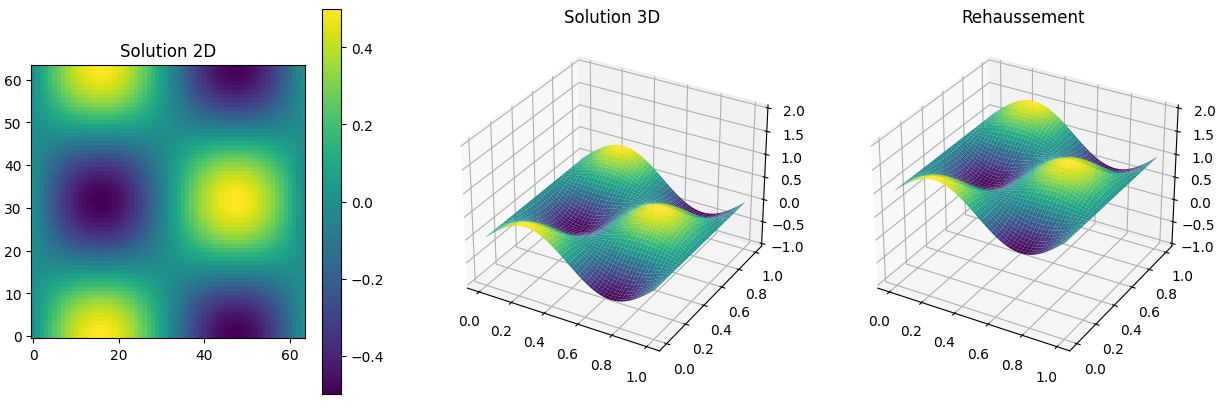
\includegraphics[width=\linewidth]{solution.png}
\end{minipage}

On se ramène alors on problème
$$\left\{\begin{aligned}
	&-\Delta (u_pC)=f \quad &&\Omega \\
	&C=1 \quad &&\Gamma
\end{aligned}\right.$$

Et donc
$$\left\{\begin{aligned}
	&-\Delta(\tilde{\phi}C)=f \quad &&\Omega \\
	&C=1 \quad &&\Gamma
\end{aligned}\right.$$

On obtient alors
$$\tilde{u}=\tilde{\phi}C$$

Et donc
$$u_C=\tilde{\phi}C-m$$

On obtient alors la formulation variationnelle suivante (avec comme fonction test $\tilde{\phi}v$) :
$$\int_{\Omega}\nabla (\tilde{\phi}C)\cdot\nabla (\tilde{\phi}v)=\int_\Omega f\tilde{\phi}v$$

Voici les résultats obtenus pour différents $m$ :

\begin{minipage}{\linewidth}
	\centering
	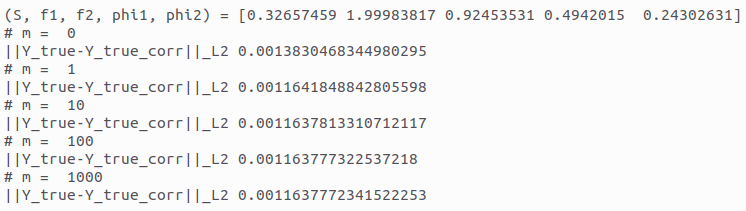
\includegraphics[width=0.8\linewidth]{resultats.png}
\end{minipage}
